In this chapter we present the numerical results of our SRG calculations and analyse and discuss them. To get an idea about the performance of the SRG method, we start with the free-space case. After making out computational challenges and methods to improve convergence, we continue with in-medium calculations. 
Here we start with Wegner's canonical generator, which as standard generator serves as first starting point to drive the Hamiltonian to a diagonal form, and identify the problems associated with this generator in our in-medium calculations. Eventually, we devote a whole section to IM-SRG(2) calculations with White's generator, with which we perform our final computations and compare the SRG with other many-body methods.\\
Note that  all results in this chapter are given in atomic units, as introduced in chapter \ref{chap:qdots}.

\section{Free-space SRG}
As a first test for the SRG method, we perform the evolution in free space. Obviously, this is computationally much less effective than the in-medium approach, since the full Hamiltonian matrix needs to be set up. However, in contrast to the in-medium evolution, the flow equations are not truncated. This in turn means that we obtain a result which is correct within the SRG approach and therefore can be used as a benchmark to measure the truncation error later on.

\subsection{Code validation}
When developing a computer program, it is crucial to test the code for errors. Large errors are usually easy to detect, since one often has an estimate for the results. Therefore it does usually not need more than a few runs to reveal that there is a bug in the code, which has to be found and correct. A much greater challenge is to identify minor bugs in the code, often leading to results that are incorrect, but still within the estimated range. \\
In order to guarantee that our implementation is free of errors, we therefore perform numerous tests where we know the exact result. Reproducing those ones, we can be sure that the tested part of program works as it is expected to do, and that this one can be used as a reliable input for further calculations.

\paragraph*{Hamiltonian matrix} 
The free-space approach of the SRG method relies on a proper setup of the Hamiltonian matrix. It is therefore essential to test that this matrix is correct. Two of the major error sources are an incorrect sign after applying the creation and annihilation operators, as well as a wrong interaction element due to incorrect spin considerations when computing direct and exchange term.\\
To test the setup of our matrix, we take the example of $N = 2$ particles and $R = 3$ shells. The correct Hamiltonian matrix is presented in \cite{Marte}, which makes it possible to compare every single element.

The considered system contains twelve singe-particle states with the following mappings \mbox{$|\alpha\rangle \rightarrow |n,m,m_s\rangle$}:
\begin{align*}
|0\rangle &\rightarrow |0,0,-1\rangle, \quad\quad |6\rangle \rightarrow |0,-2,-1\rangle \\
|1\rangle &\rightarrow |0,0,+1\rangle, \quad\quad |7\rangle \rightarrow |0,-2,+1\rangle \\
|2\rangle &\rightarrow |0,-1,-1\rangle, \quad |8\rangle \rightarrow |0,+2,-1\rangle \\
|3\rangle &\rightarrow |0,-1,+1\rangle, \quad |9\rangle \rightarrow |0,+2,+1\rangle \\
|4\rangle &\rightarrow |0,+1,-1\rangle, \quad |10\rangle \rightarrow |0,0,-1\rangle \\
|5\rangle &\rightarrow |0,+1,+1\rangle, \quad |11\rangle \rightarrow |0,0,+1\rangle .\\
\end{align*}

As explained in chapter \ref{chap:qdots}, the Hamiltonian does only connect states with the same quantum numbers $M$ and $M_s$, resulting in a block-diagonal form. Since we are mainly interested in the ground state energy, we set $M = M_s = 0$ and obtain the following possible Slater determinants as basis for the Hamiltonian matrix:
\[
|0,1\rangle,\quad |0,11\rangle,\quad |1,10\rangle,\quad |2,5\rangle,\quad |3,4\rangle,\quad |6,9\rangle, \quad|7,8\rangle,\quad |10,11\rangle.
\]
In this basis, the Hamiltonian matrix has the following form:
{\scriptsize
\setlength\arraycolsep{1pt}
\[
H=\!\left[\!
\begin{array}{cccccccc}
\langle 0,\!1| \hat{H}| 0,\!1\rangle\! &\langle 0,\!1| \hat{H}| 0,\!11\rangle &\langle 0,\!1| \hat{H}| 1,\!10\rangle & \langle 0,\!1| \hat{H}| 2,\!5\rangle&\langle 0,\!1| \hat{H}| 3,\!4\rangle &\langle 0,\!1| \hat{H}| 6,\!9\rangle & \langle 0,\!1| \hat{H}| 7,\!8\rangle& \langle 0,\!1| \hat{H}| 10,\!11\rangle\\
\langle 0,\!11| \hat{H}| 0,\!1\rangle\!& \ddots&\dots &\dots &\dots &\dots &\dots & \langle 0,\!11| \hat{H}| 10,\!11\rangle\\
\langle 1,\!10| \hat{H}| 0,\!1\rangle\!& \vdots & \ddots& & & & & \langle 1,\!10| \hat{H}| 10,\!11\rangle\\
\langle 2,\!5| \hat{H}| 0,\!1\rangle\!& \vdots & &\ddots & & & & \langle 2,\!5| \hat{H}| 10,\!11\rangle\\
\langle 3,\!4| \hat{H}| 0,\!1\rangle\!& \vdots & & & \ddots& & &\langle 3,\!4| \hat{H}| 10,\!11\rangle \\
\langle 6,\!9| \hat{H}| 0,\!1\rangle\!& \vdots & & & &\ddots & & \langle 6,\!9| \hat{H}| 10,\!11\rangle\\
\langle 7,\!8| \hat{H}| 0,\!1\rangle\!& \vdots & & & & &\ddots & \langle 7,\!8| \hat{H}| 10,\!11\rangle\\
\langle 10,\!11| \hat{H}| 0,\!1\rangle\!& \langle 10,\!11| \hat{H}| 0,\!11\rangle&\langle 10,\!11| \hat{H}| 1,\!10\rangle &\langle 10,\!11| \hat{H}| 2,\!5\rangle & \langle 10,\!11| \hat{H}| 3,\!4\rangle& \langle 10,\!11| \hat{H}| 6,\!9\rangle& \langle 10,\!11| \hat{H}| 7,\!8\rangle& \langle 10,\!11| \hat{H}| 10,\!11\rangle\\
\end{array}
\;\right]
\]}

With our Hamiltonian (\ref{eq:imsrg1}) and oscillator frequency $\omega = 1.0$, this matrix should read \cite{Marte}
{\small
\[
H = \left[
\begin{array}{cccccccc}
3.2533  & 0.3133 & -0.3133 &  0.3133 & -0.3133  & 0.1175 & -0.1175 &  0.2350\\
  0.3133  & 4.8617 & -0.2350&  -0.0783 &  0.0783  &-0.0881&   0.0881&  0.1371\\
  -0.3133 & -0.2350 &  4.8617&  0.0783 & -0.0783  & 0.0881 & -0.0881 & -0.1371\\
   0.3133  &-0.0783&   0.0783  & 4.8617&  -0.2350 &  0.3035 & -0.1469 &  0.1371\\
  -0.3133  & 0.0783 & -0.0783 & -0.2350 &  4.8617 & -0.1469 &  0.3035 & -0.1371\\
   0.1175  &-0.0881 &  0.0881 &  0.3035  &-0.1469  & 6.7160 & -0.1285  & 0.1395\\
  -0.1175  & 0.0881 & -0.0881 & -0.1469   &0.3035 & -0.1285  & 6.7160 & -0.1395\\
   0.2350 &  0.1371 & -0.1371 &  0.1371  &-0.1371&   0.1395  &-0.1395&   6.7491\\
\end{array}
\right].
\]
}
This matrix is exactly reproduced by our code, proving the correct setup of the Hamiltonian. 

\paragraph*{Diagonalization}
In order to make statements about the accuracy of the SRG method, we will compare our results  with the ones obtained by exact diagonalization. For the small systems considered with the free-space approach, it is efficient enough to do this with the standard function \textit{eig\_sym} of the Armadillo library \cite{Armadillo}. For the above Hamiltonian matrix, this function returns the lowest eigenvalue\\
\[
E_0 = 3.0386,
\]
which is in accordance to \cite{Marte}. For two shells, we expect \cite{Christoffer}
\[
E_0 = 3.1523,
\]
which is also reproduced. As in the rest of the thesis, the energy is given in units of $\left[ E_H \right]$. The last two results imply that also this diagonalizing function is correctly applied and can be relied on when benchmarking the SRG results.

\subsection{Numerical results}
Having verified that the SRG routine obtains the correct input matrix, we perform runs for systems of different size and oscillator frequency $\omega$.

As a first approach, we take a harmonic oscillator basis and study the convergence behaviour using a standard Coulomb interaction.\\
In atomic units, the Hamiltonian of the two-dimensional parabolic quantum dot for this standard interaction reads
\be 
\hat H = \sum_{i=1}^N \left(-\frac{1}{2}\nabla_i^2 + \frac{1}{2} \omega^2r_i^2\right) + \sum_{i<j} \frac{1}{r_{ij}},
\ee 
see section \ref{sec:ModHam}.
The oscillator frequency $\omega$ is used to tune the confining
potential, which means the higher $\omega$ is, the more confined
the particles are. Mathematically, the complete non-interacting energy $E_{non} = \sum\limits_i\epsilon_i = \omega\sum\limits_i \lb 2n + |m_l| + 1\rb$ is proportional to $\omega$, whereas the oscillator frequency has no significant impact on the interaction energy. This means that the influence of the interaction energy, contributing to the potential energy, diminishes for larger values of $\omega$, leading to a relative increase of the kinetic energy. Experimentally, the frequency can be tuned, too, which allows to analyse the system in terms of different frequencies. For this reason, we perform all our numerical calculations with different values of $\omega$ and study how the frequency is affecting the results, as well as the numerical stability of the SRG method.

As introduced in section \ref{sec:ChoiceEta}, the two most fundamental generators are 
\be
\hat{\eta}_1 = \left[\hat{T}_{\text{rel}},\hat{V}\right]
\ee
and Wegner's original choice
\be
 \hat{\eta}_2 = \left[\hat{H}^{\rm d},\hat{H}^{\rm od}\right],
\ee
where we suppress the $s$-dependence for simplicity and label them as $\hat{\eta}_1, \hat{\eta}_2$ for easy access later on. 

In order to compare their effect on the flow of the Hamiltonian, we perform calculations with both generators. Tables \ref{tab:free1} and \ref{tab:free2} display the results for systems with two, six and twelve electrons and compare them to the result obtained with exact diagonalization (FCI).

\begin{table}
\begin{center}
\begin{tabular}{|c|c|c|c|c|}
\hline\hline
$\omega$ &R & $\hat{\eta}_1$ & $\hat{\eta}_2$ & FCI \\
\hline
  0.1    & 2 &  0.5125198414    & 0.5125198414   & 0.5125198414             \\
         & 4 & 0.4418679942     &  0.4418679942   & 0.4418679942         \\
         & 6 & 0.441446672      & 0.441446672    & 0.441446672           \\
         & 8 & 0.4412461536    & 0.4412461536    & 0.4412461536             \\
         & 10& 0.441135127     &0.441135127     & 0.441135127               \\ 
\hline    
  0.28   & 2 &  1.127251038    & 1.127251038   & 1.127251038        \\
         & 4 & 1.028803672     & 1.028803672   & 1.028803672            \\
         & 6 & 1.025448813     & 1.025448813   & 1.025448813          \\
         & 8 & 1.024199606    & 1.024199606      & 1.024199606          \\
         & 10& 1.023550577    & 1.023550577    & 1.023550577           \\  
\hline 
  0.5   & 2 & 1.78691353      & 1.78691353   &  1.78691353          \\
        & 4 & 1.673872389    & 1.673872389    & 1.673872389         \\
        & 6 & 1.667257181    & 1.667257181    & 1.667257181        \\
        & 8 & 1.664806939    & 1.664806939    & 1.664806939        \\
        & 10& 1.663535219    & 1.663535219       & 1.663535219          \\ 
\hline   
  1.0    & 2 & 3.152328007    & 3.152328007    & 3.152328007      \\
         & 4 &  3.025230582   & 3.025230582    & 3.025230582          \\
         & 6 & 3.013626129    & 3.013626129    & 3.013626129           \\
         & 8 & 3.009235721 & 3.009235721 & 3.009235721           \\
         & 10& 3.006937178   & 3.006937178     & 3.006937178      \\    
 \hline\hline
 \end{tabular}
\end{center}
\caption{The ground state energy $E_0$ (in $\left[E_H\right]$) for $N=2$ particles is compared between generator $\hat{\eta}_1 = \left[ \hat{T}_{\text{rel}}, \hat{V}\right]$, generator  $\hat{\eta}_2 = \left[ \Hd, \Ho \right]$ and exact diagonalization (FCI). The large number of specified digits shall demonstrate that exactly the same results are obtained. This table is just an excerpt, the full table \ref{tab:full1} can be found in Appendix \ref{App:AppendixA}.}
\label{tab:free1}
\end{table}


\begin{table}
\begin{center}
\begin{tabular}{|c|c|c|c|c|c|}
\hline\hline
N&$\omega$ &R & $\hat{\eta}_1$ & $\hat{\eta}_2$ & FCI \\
\hline
6 &  0.1    & 3 & 4.149558313  & 4.149558313  & 4.149558313  \\
 &         & 4 & 3.797435926  &    nc          & 3.797435926  \\ 
 \cline{2-6}    
 &  0.28   & 3 &   nc   &  nc &  8.518319500  \\
 &         & 4 &  7.851831187  & nc  &   7.851831187   \\
  \cline{2-6}
 &  0.5   & 3 &   12.89722859    & 12.89722859   &  12.89722859         \\
&         & 4 &  12.03694209  & nc &     12.03694209   \\
 \cline{2-6} 
 &  1.0    & 3 & 21.42058830    & 21.42058830  &  21.42058830     \\  
 &         & 4 & 20.41582765   &  nc  &   20.41582765   \\
\hline
12 & 1.0 & 4 & 70.31250219 &70.31250218 & 70.31250218 \\
\cline{2-6} 
  & & & & & 43.29176947 \\
 \hline\hline
 \end{tabular}
\end{center}
\caption{Comparison of the ground state energy $E_0$ as in table \ref{tab:free1}. The label ''nc'' denotes non-converging runs. TODO: maybe some more examples for 12 particles}
\label{tab:free2}
\end{table}

As can be seen in both tables, both generators reproduce precisely the ground state energy which can be obtained by exact diagonalization of the Hamiltonian matrix. In other words, the ground state seems to get completely  decoupled from the other matrix elements. However, Wegner's choice of the generator $\hat{\eta}_2 = \left[ \Hd, \Ho \right]$ seems to be numerically more unstable and results more often in a non-converging ground state energy. 

Since this is also of great importance later on, it should be demonstrated what we mean by converging and non-converging simulations:\\
 Figure \ref{fig:convComp} shows some typical examples:
In plots $(a)$ and $(b)$, the ground state energy $E_0$ is monotonically decreasing during the whole integration procedure and finally stabilizing at a constant value. Just if we integrate extremely close to $\lambda=0$, in some cases numerical instabilities let $E_0$ suddenly explode to very large values again. However, this happens after a clear convergence on a longer interval and is not of physical relevance. On the other hand, with an increasing number of particles and a lower oscillator frequency $\omega$, we often obtain  results like examples $(c)$ and $(d)$ in figure \ref{fig:convComp}. In plot $(c)$, the energy increases again without having stabilized at a constant value before, and in plot $(d)$, it does not decrease at all. Since the method theoretically should converge, we suspect that numerical instabilities in the ODE solver are responsible for this effect. The  convergence behaviour will be discussed more thoroughly in subsection \ref{subsec:FreeEffAndHF}.

\begin{figure}
\begin{center}
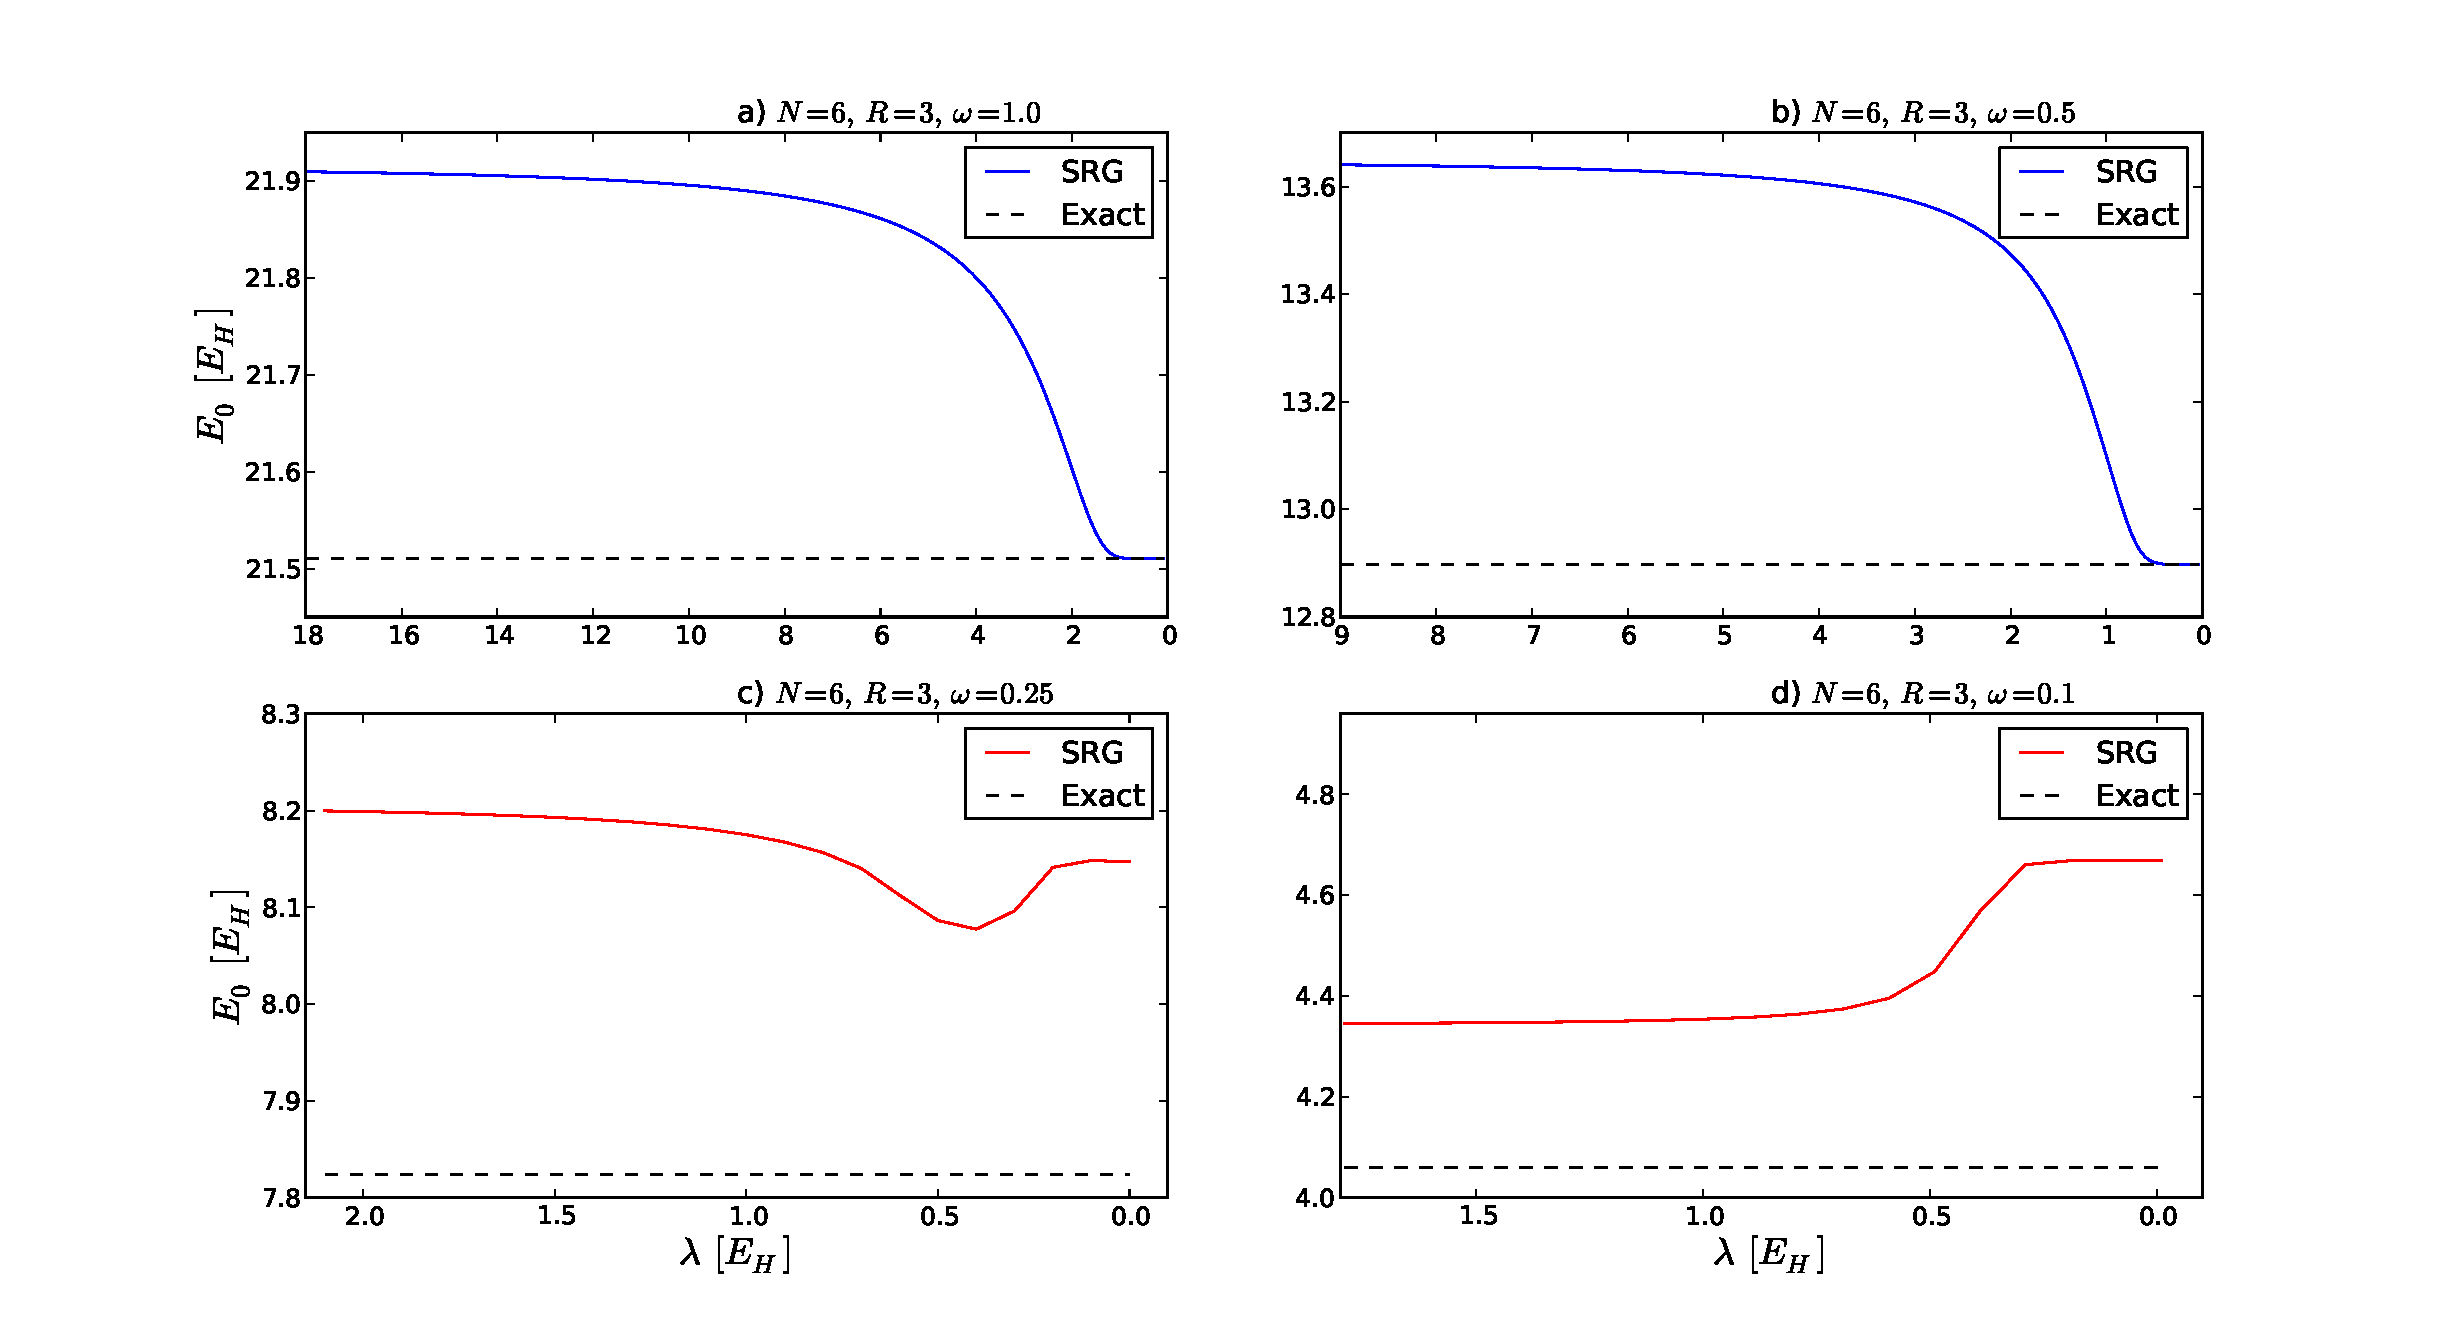
\includegraphics[scale=0.42]{../Plots/convComp.pdf}
\caption{Typical plots demonstrating the obtained behaviour of the ground state energy for converging ($(a)$ and $(b)$ and non-converging cases ($(c)$ and $(d)$. In these plots, generator $\hat{\eta}_2 = \left[ \Hd, \Ho \right]$ has been used, but the figure illustrates likewise curves for converging and non-converging runs if  generator $\hat{\eta}_1 = \left[ \hat{T}_{\text{rel}}, \hat{V}\right]$ is used. }
\label{fig:convComp}
\end{center}
\end{figure}

Having found out that, in general, generator $\hat{\eta}_1 = \left[ \hat{T}_{\text{rel}}, \hat{V}\right]$ yields more often a converging result, we were interested in those cases where both generators lead to a converging $E_0$, and have analysed whether there exist qualitative differences in the flow, too. 

\begin{figure}
\begin{center}
\subfigure{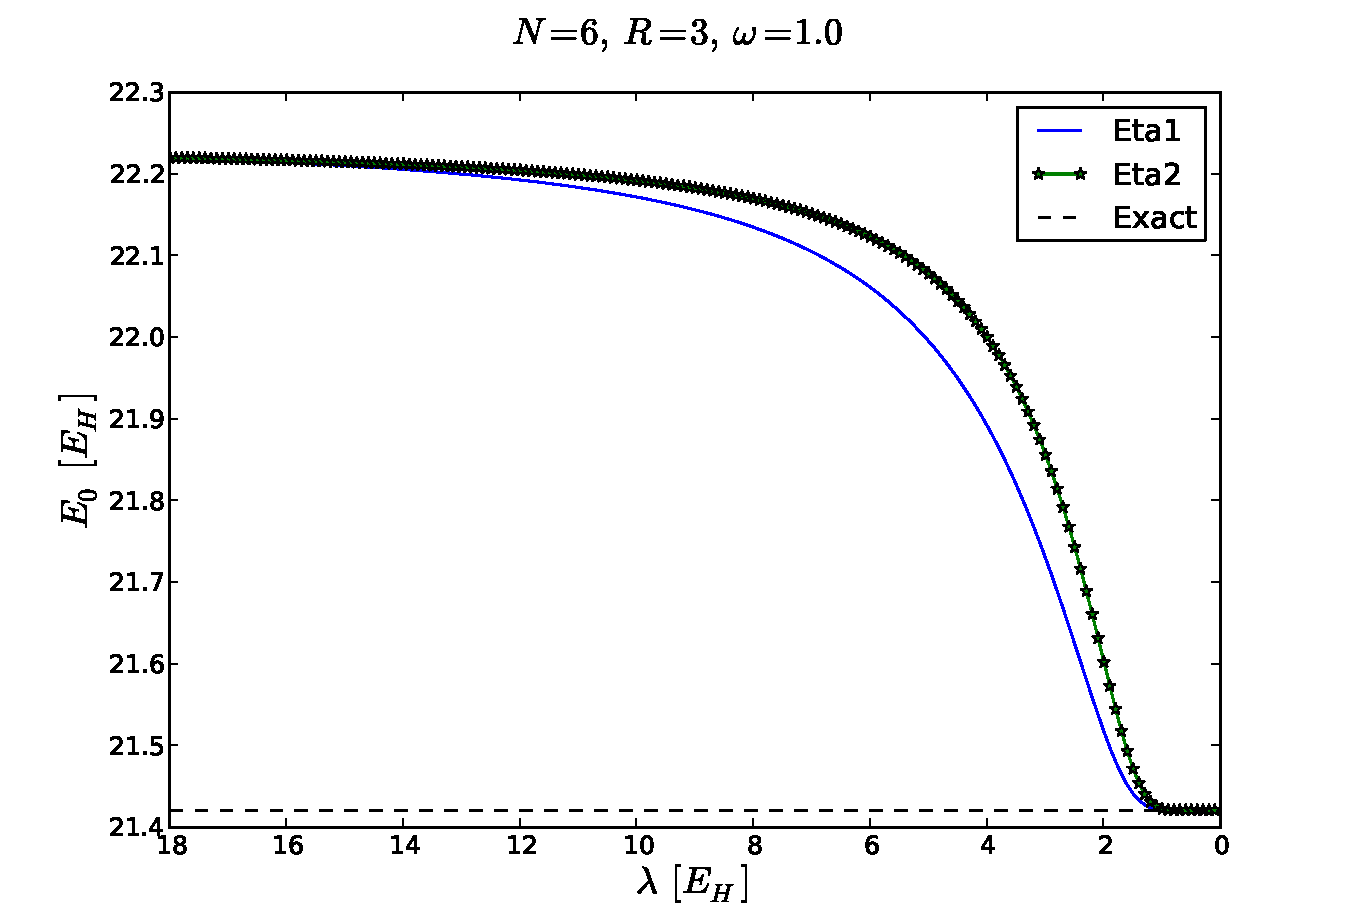
\includegraphics[scale=0.33]{../Plots/etaComp.pdf}}
\subfigure{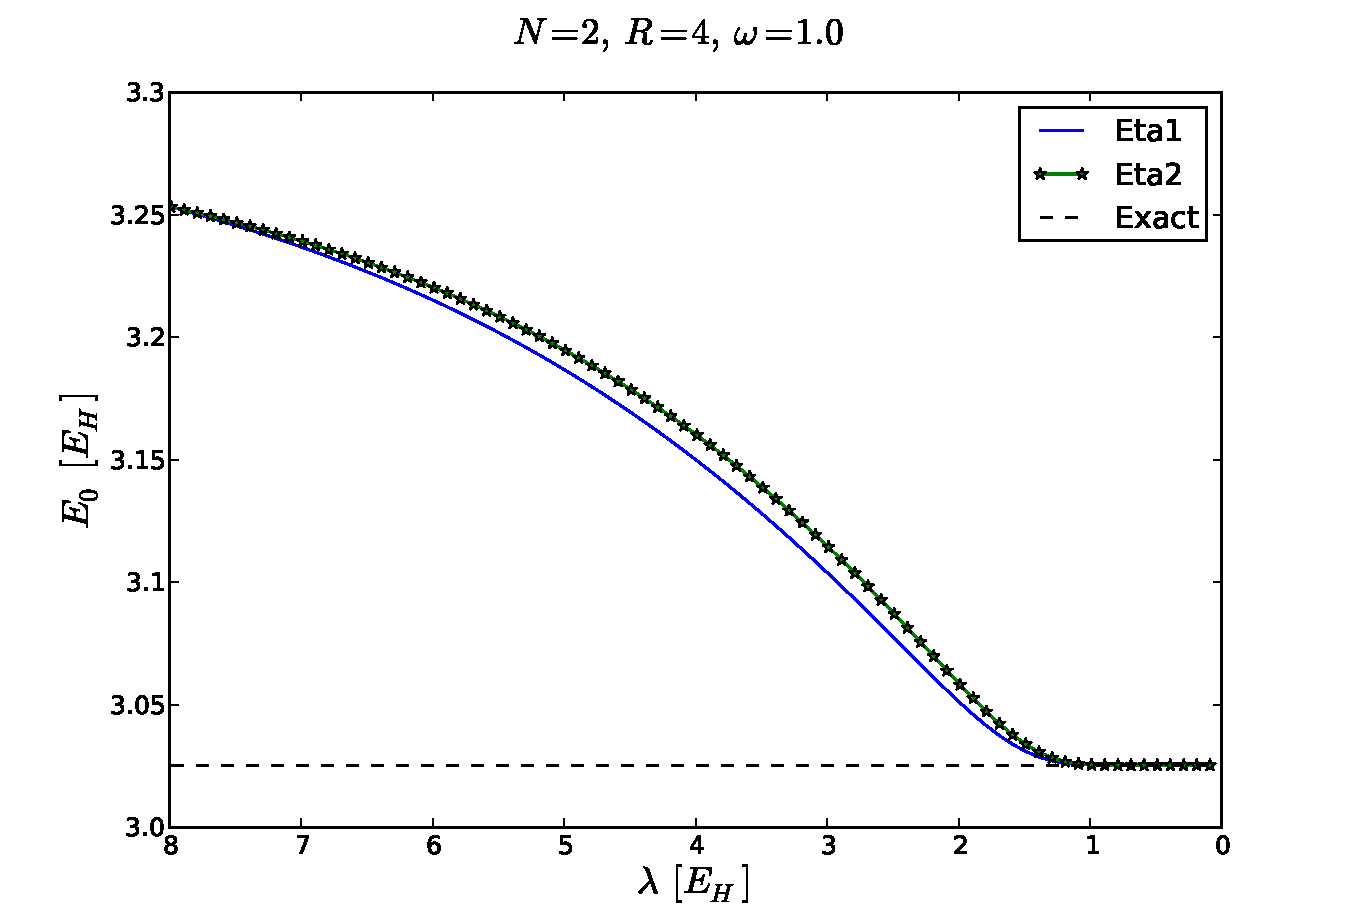
\includegraphics[scale=0.34]{../Plots/etaComp2.pdf}}
\end{center}
\caption{Comparison of the convergence behaviour of the the two generators $\hat{\eta}_1 = \left[ \hat{T}_{\text{rel}}, \hat{V}\right]$ and $\hat{\eta}_2 = \left[ \Hd, \Ho \right]$. Although both generators lead to a converging result and convergence sets in at approximately the same value of $\lambda$, decoupling appears to be faster for $\hat{\eta}_1$.}
\label{fig:EtaComp}
\end{figure}

Figure \ref{fig:EtaComp} shows two typical results: Although the final point of convergence is reached for approximately the same value of $\lambda$, it is noticeable that the curve of generator $\hat{\eta}_1 = \left[ \hat{T}_{\text{rel}}, \hat{V}\right]$ constantly lies below the one of  $\hat{\eta}_2 = \left[ \Hd, \Ho \right]$. This in turn means that even in the converging case, generator $\hat{\eta}_1$ seems  to lead to a better and faster decoupling for the studied quantum dots.


In order to verify the decoupling of the ground state energy by the SRG method and to illustrate how the Hamiltonian is driven to a diagonal form during the flow, we have made snapshots of the Hamiltonian matrix at different stages of the integration process. Since the non-interacting part of the Hamiltonian already is in diagonal form and those elements dominate the plots, we have chosen to restrict us to the interaction elements. A typical evolution for the case of $N=2$ particles and $R = 4$ shells is shown in figure \ref{fig:HamilFlow}.

\begin{figure}
\subfigure{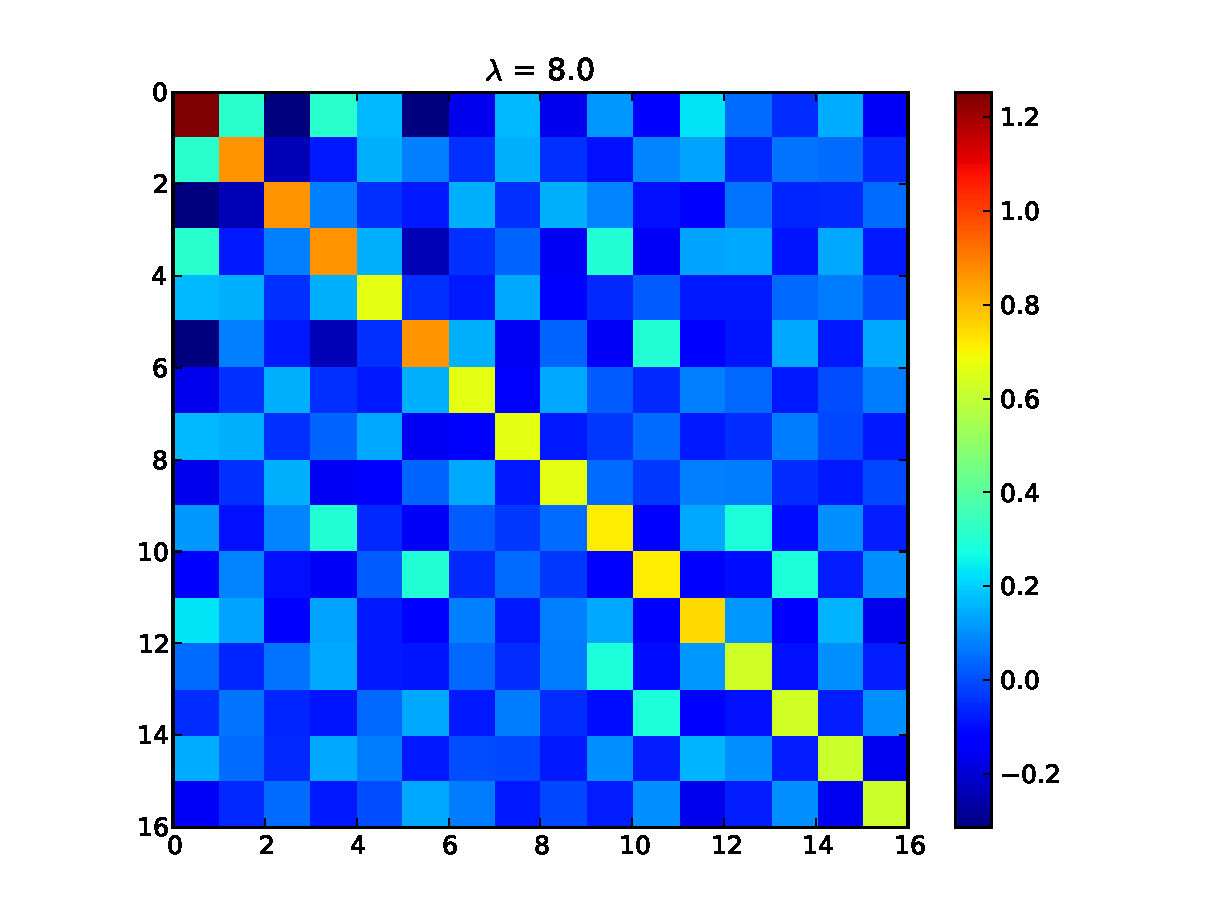
\includegraphics[scale=0.246]{../Plots/Hstart.pdf}}
\subfigure{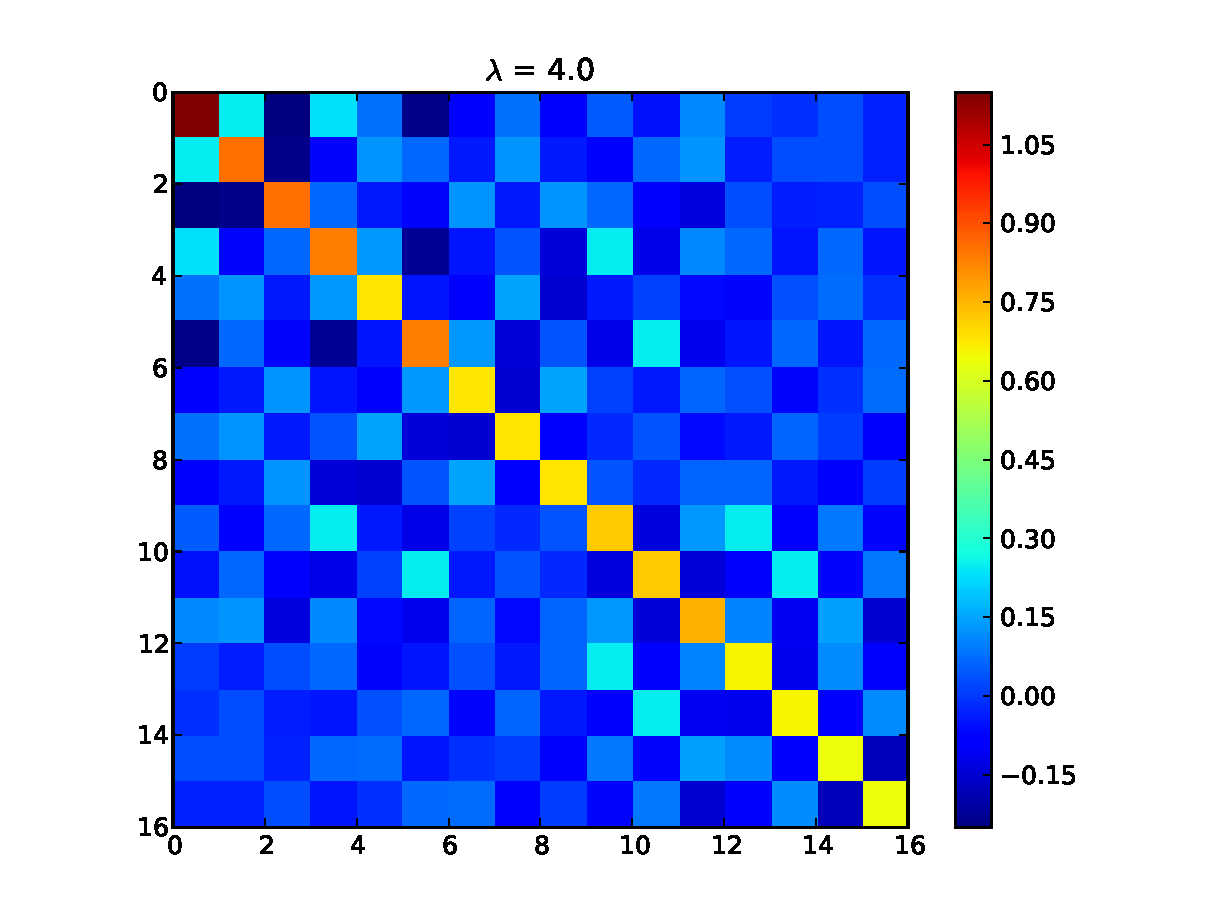
\includegraphics[scale=0.247]{../Plots/H4.pdf}}
\subfigure{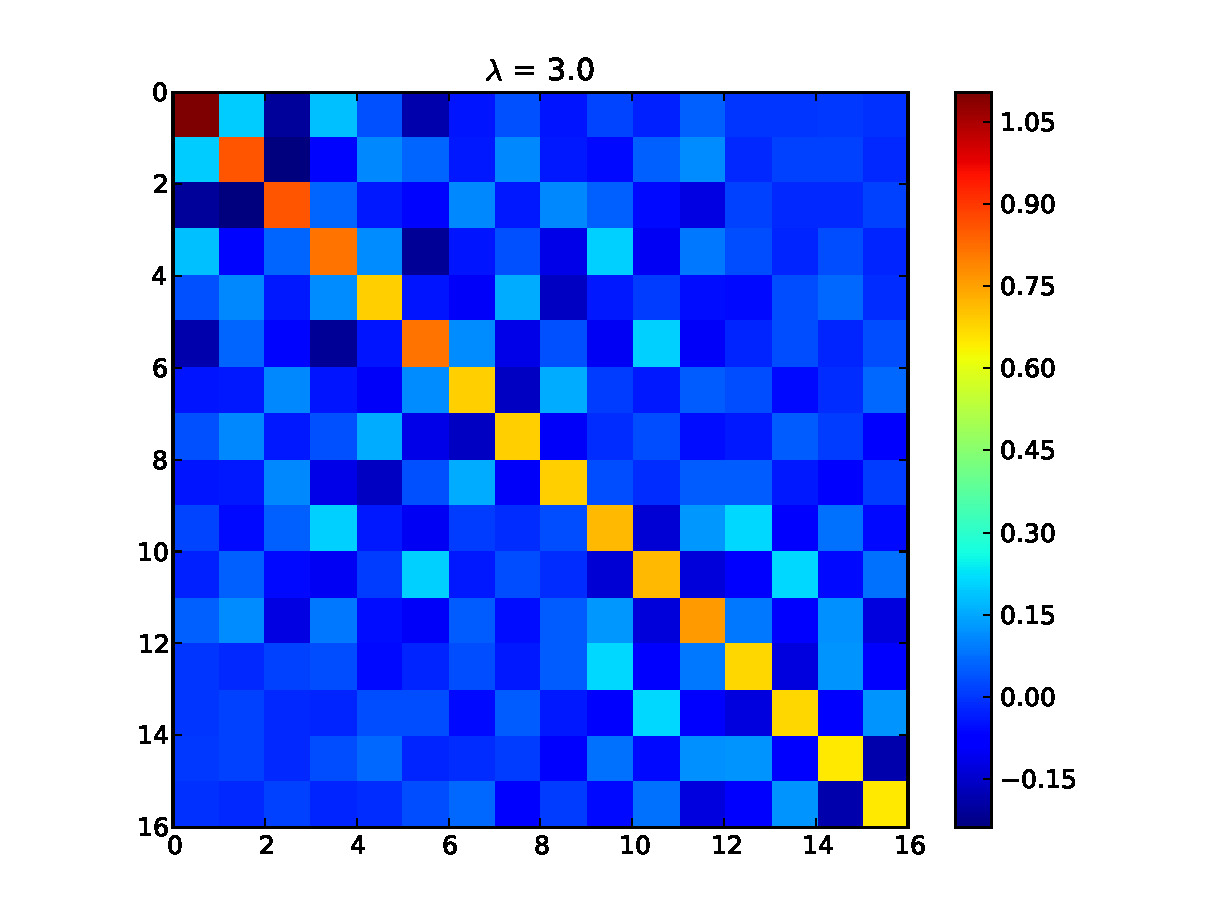
\includegraphics[scale=0.247]{../Plots/H3.pdf}}
\subfigure{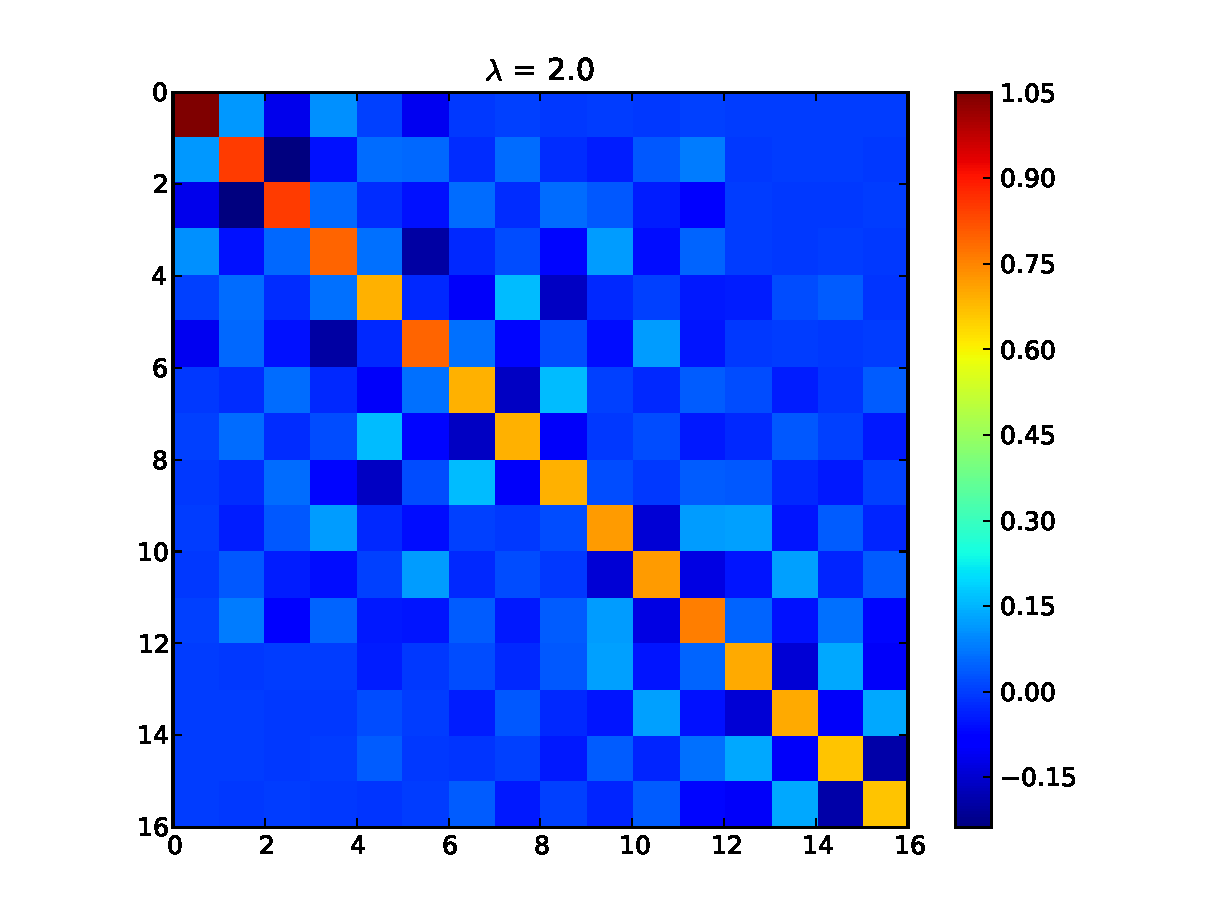
\includegraphics[scale=0.247]{../Plots/H2.pdf}}
\subfigure{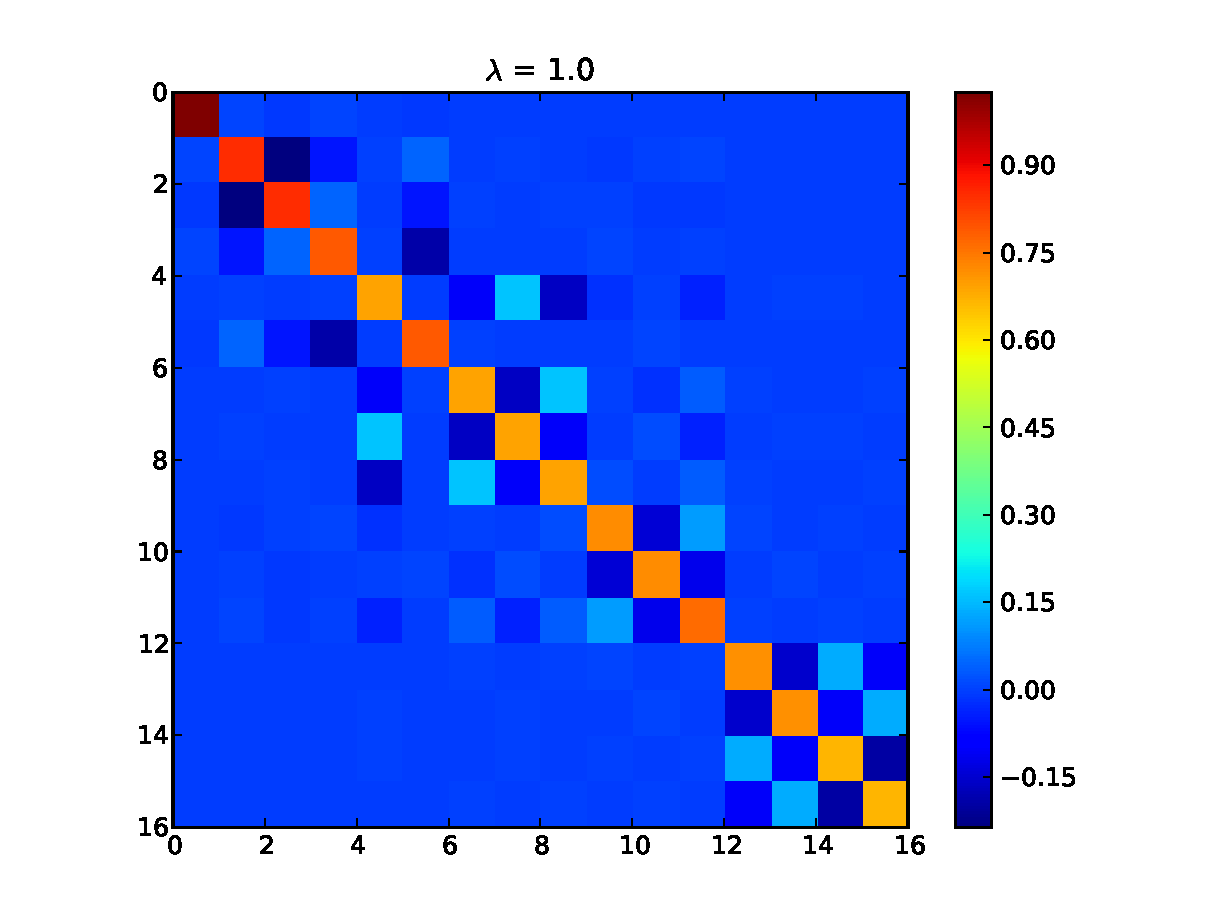
\includegraphics[scale=0.246]{../Plots/H1.pdf}}
\subfigure{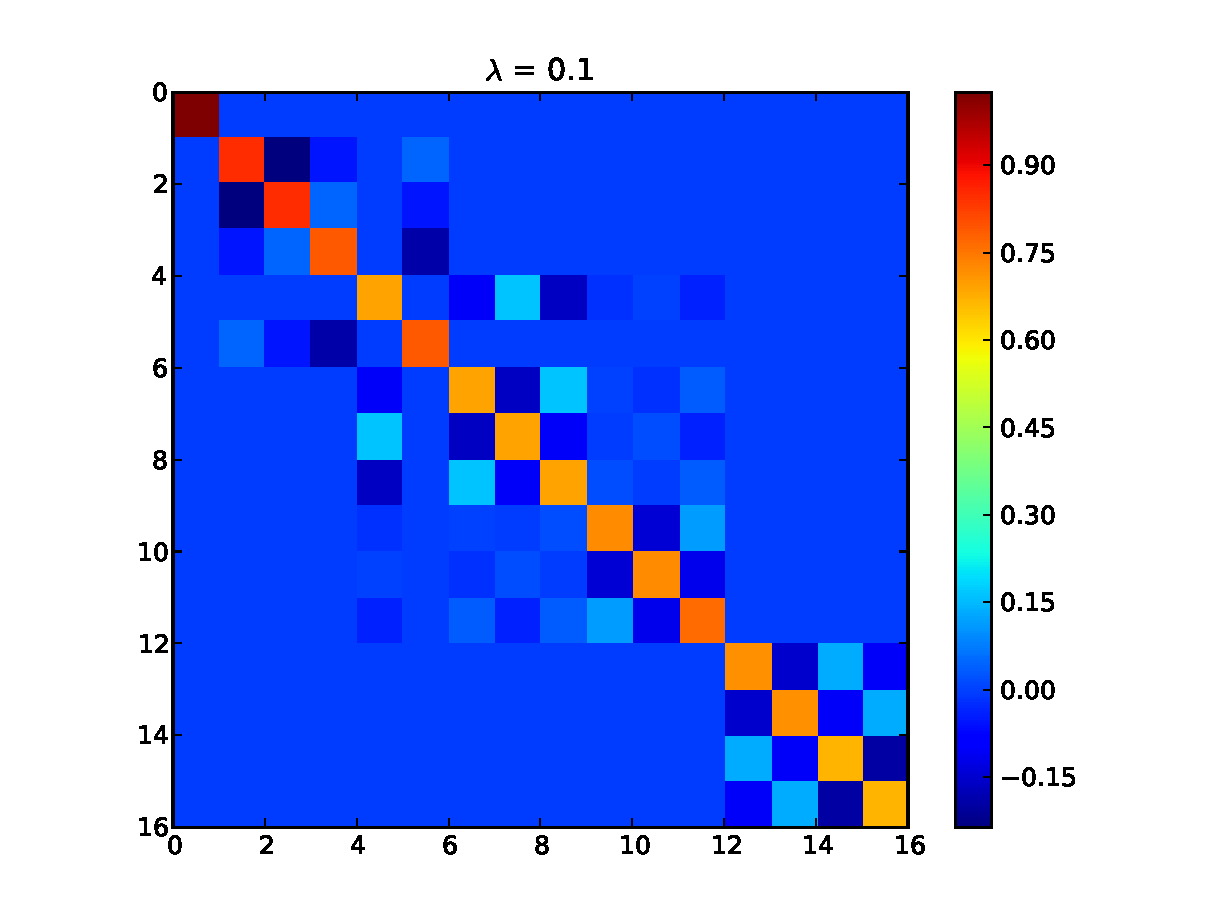
\includegraphics[scale=0.246]{../Plots/H01.pdf}
}
\caption{Snapshots of the interaction elements of the  Hamiltonian matrix at different stages of the flow, specified by the flow parameter $\lambda$. The evolution is show for a system of $N=2$ particles, $R = 4$ shells, oscillator frequency $\omega=1.0$ and generator $\hat{\eta}_1 = [\hat{T}_{\text{rel}},\hat{V}]$.}
\label{fig:HamilFlow}
\end{figure}

The Hamiltonian matrix behaves exactly as expected: At the beginning of the flow, we have non-zero elements at all places of the matrix. During the flow, first the elements which are far off the diagonal are zeroed out, followed by the ones closer to the diagonal. This is especially well illustrated in the transition from the fourth to the fifth plot, corresponding to $\lambda = 2.0$ and $\lambda = 1.0$, respectively. Note that in the whole thesis, we have that $\left[ \lambda \right] = \left[E\right ] = E_H$ due to $\lambda = s^{-1/2}$. In the case of $\lambda = 2.0$, just the matrix elements connecting states with highest possible energy differences seem to be close to zero, while in the plot for $\lambda = 1.0$, this is true for a much greater area of the matrix's upper and lower triangular part. Finally, in the last plot, the ground state seems to be completely decoupled from the remaining states. Even if not the whole interaction is completely diagonal, this should mean that the energy at that stage should have converged to its final value.\\
\begin{figure}
\begin{center}
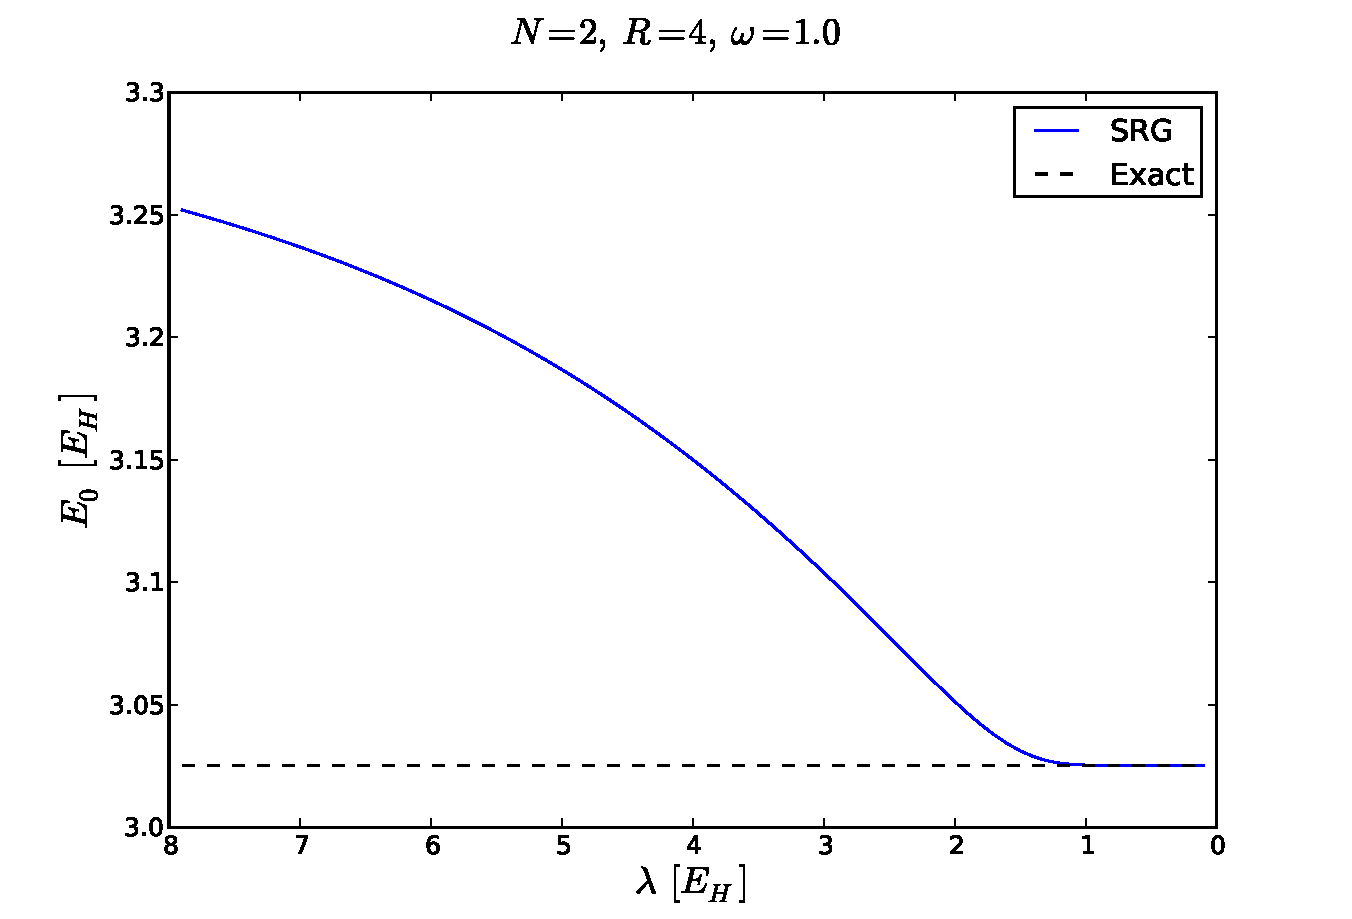
\includegraphics[scale=0.4]{../Plots/energy1.pdf}
\end{center}
\caption{Evolution of the ground state energy for a system with $N=2$ particles, $R = 4$ shells, oscillator frequency $\omega=1.0$ and generator $\hat{\eta}_1 = [\hat{T}_{\text{rel}},\hat{V}]$.}
\label{fig:energy1}
\end{figure}
In order to confirm this statement, we have plotted the evolution of the ground state energy for this example in figure \ref{fig:energy1}. From $\lambda = 8.0$ down to $\lambda = 1.0$, we know from figure \ref{fig:HamilFlow} that many matrix elements are zeroed out and, correspondingly, a large drop can be observed for the ground state energy $E_0$. Afterwards, the Hamiltonian matrix in figure \ref{fig:HamilFlow} does only slightly change and seems to have converged to its final shape for $\lambda = 0.1$. Analogously, we observe a more or less constant value for $E_0$. Thus, the latter one reflects very well the behaviour of the whole Hamiltonian.
 
An interesting aspect of figure \ref{fig:HamilFlow} are the groups of three to four states which the SRG method seems not to be able to zero out. To explain this phenomenon, it is necessary look at the involved Slater determinants. Table \ref{tab:SDs} lists for each Slater determinant $|\alpha\rangle$ the two occupied singe-particle states, as well as the sum of both single-particle energies $\Sigma_{\alpha} = \epsilon_1 + \epsilon_2$.\\
\begin{table}
\begin{center}
\begin{tabular}{cc|cc}
\hline\hline
$|\alpha\rangle$ & $\Sigma_{\alpha}$ & $|\alpha\rangle$ & $\Sigma_{\alpha}$\\
\hline
$|0,1\rangle$ & $2\omega$ & $|5,16\rangle$ & $6\omega$ \\
$|0,11\rangle$ & $4\omega$ & $|6,9\rangle$ & $6\omega$ \\
$|1,10\rangle$ & $4\omega$ & $|7,8\rangle$ & $6\omega$ \\
$|2,5\rangle$ & $4\omega$ & $|10,11\rangle$ & $6\omega$ \\
$|2,19\rangle$ & $6\omega$ & $|12,15\rangle$ & $8\omega$ \\
$|3,4\rangle$ & $4\omega$ & $|13,14\rangle$ & $8\omega$ \\
$|3,18\rangle$ & $6\omega$ & $|16,19\rangle$ & $8\omega$ \\
$|4,17\rangle$ & $6\omega$ & $|17,18\rangle$ & $8\omega$ \\
\hline\hline
\end{tabular}
\end{center}
\caption{Slater determinant basis for a system with $N=2$ particles and $R = 4$ shells. The sum of the single-particle energies of both particles, $\Sigma_{\alpha} = \epsilon_1 + \epsilon_2$, is given in units of  $\left[ E_h \right]$. The single-particle states are indexed as in figure \ref{fig:shellstructure}}.
\label{tab:SDs}
\end{table}
The table illustrates that many of the Slater determinants are energetically degenerate. Beginning with the states with highest energy, the first degeneracy involves the last four states. The effect on figure \ref{fig:HamilFlow} is, that the last $4\times 4$ block of the Hamiltonian does not converge to a diagonal form. Further on, the next set of degenerate states is formed by the six determinants $|3,18\rangle$ to $|10,11\rangle$. Relating this to the plots of figure \ref{fig:HamilFlow}, we see that also these six states result in a non-zero block, which additionally is much more pronounced for clusters of $3 \times 3$ blocks. Taking account the shell structure of figure \ref{fig:shellstructure}, we see that for the first three states of this $6 \times 6$ block, the particle occupy single-particle states of different shells, namely $R = 2$ and $R=4$. For the remaining three states, all particles occupy the same shell $R = 3$. \\
All the named correspondences between table \ref{tab:SDs} and figure \ref{fig:HamilFlow} show that the final shape of the Hamiltonian matrix depends very much on the structure of the system and that energy degeneracies result in non-diagonal blocks. 

In order to see the block-diagonal form in a more intuitive way, one needs to exchange states $|2,19\rangle$ and $|3,4\rangle$, which unfortunately have been arranged in the wrong way considering energy $\Sigma_{\alpha}$. With this arrangement, the final Hamiltonian looks as in figure \ref{fig:HamilOrdered}, clearly illustrating the block-diagonal form due to energy degeneracies.
\begin{figure}
\begin{center}
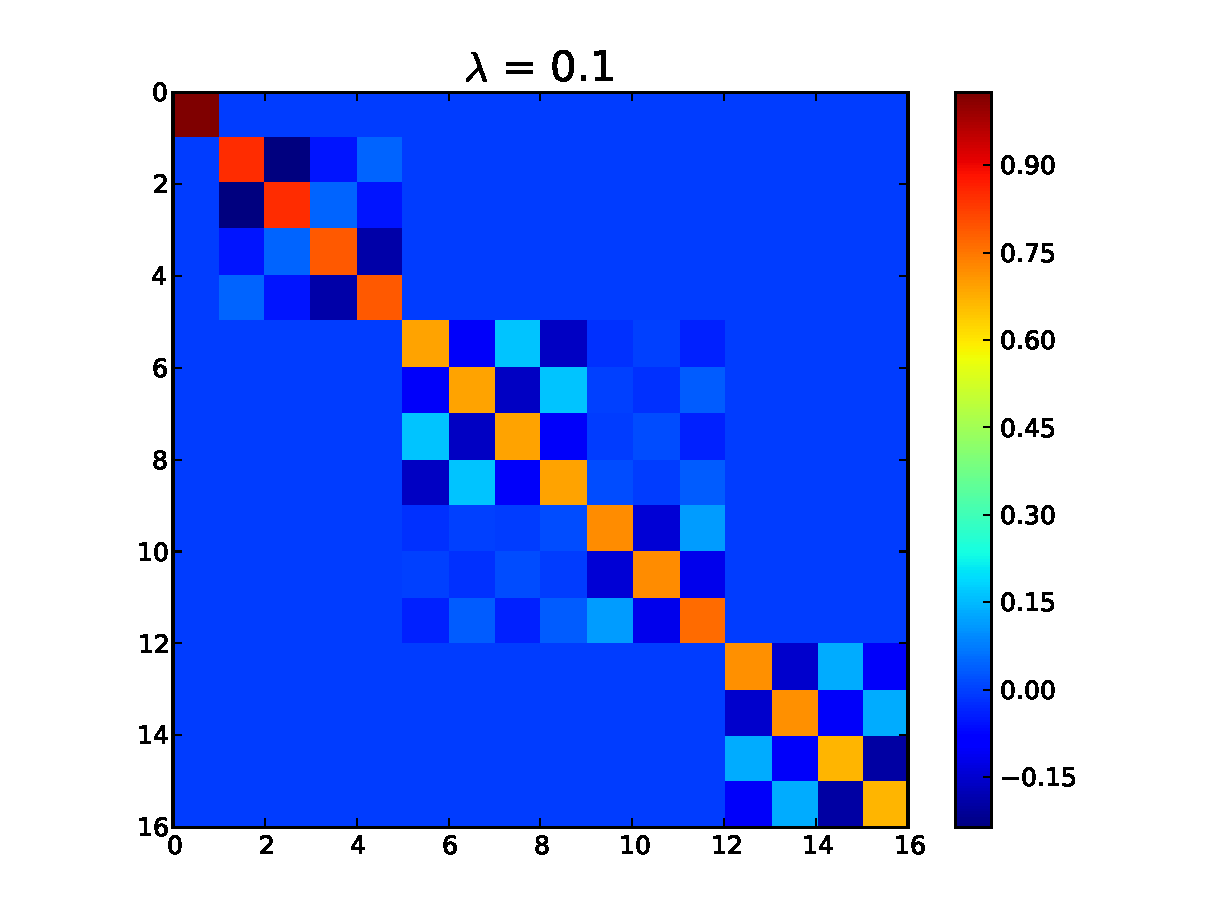
\includegraphics[scale=0.35]{../Plots/HamiltonPlotOrdered.pdf}
\end{center}
\caption{Interaction elements of the Hamiltonian for a system of $N=2$ particles, $R=4$ shells and $\omega=1.0$. Snapshot of the evolution at $\lambda = 0.1$. Compared to figure \ref{fig:HamilFlow}, the basis states are explicitly ordered by increasing energy, pointing out the block-diagonal form of the final Hamiltonian.}
\label{fig:HamilOrdered}
\end{figure}
The behaviour can easily be explained by looking at the first-order solution of the flow equations, Eq. (\ref{eq:flowdemo}), which we restate here:
\be
V_{ij}(s) \approx V_{ij}(0) \text{e}^{-s (\epsilon_i - \epsilon_j)^2}.
\label{eq:flowdemo1}
\ee
Until now, we argued that the off-diagonal elements are zeroed out the faster, the larger the energy difference $(\epsilon_i - \epsilon_j)$ between the corresponding bra- and ket-state is. In figures \ref{fig:HamilFlow} and \ref{fig:HamilOrdered} the extreme case is illustrated, namely that an energy degeneracy of two or more states prevents the interaction connecting those states to 
converge quickly to zero. This is valid for Wegner's choice of the generator $\hat{\eta}_2 = \left[ \Hd, \Ho \right]$, as well as $\hat{\eta}_1 = \left[ \hat{T}_{\text{rel}}, \hat{V}\right]$. \\
In the case of quantum dots, however, we do not expect this to have impact on the ground state \mbox{energy $E_0$}, since that one is uniquely defined without degeneracy of several states. The fact that $E_0$ converges to the  same value as an exact diagonalization results in, underlines and verifies this assumption. For more complicated  systems, however, one should keep this fact in mind, and possibly draw on different generators.


\subsection{Improving convergence: Effective interaction and Hartree-Fock basis}
\label{subsec:FreeEffAndHF}

Especially as the frequency $\omega$ is lowered, we often encounter cases with a non-converging ground state energy $E_0$. In the following, we will try two methods to improve convergence and analyse how the result is affected. First, we will exchange the standard interaction by a more advanced effective interaction and compare the results. Afterwards, we will make use of a Hartree-Fock basis and examine how $E_0$ converges with this basis.


\subsubsection{Effective Interaction}

Up to this point, we have used the Coulomb interaction as so-called \textit{standard interaction}. Since this one has a divergency at $r=0$, convergence is rather slow as function of $R$ if a harmonic oscillator basis is used. \\
A common way to solve this problem is to introduce a renormalized Coulomb interaction, called \textit{effective interaction}. The effective interaction aims to speed up the convergence rate as function of the numbers of shells $R$. It has been widely used first in nuclear physics, and later on also for quantum dots \cite{PhysRevB.84.115302}.

The basis idea is to  look at a model space $\mathcal{P}$ of smaller dimension $m$ than the full $n$-dimensional Hilbert space $\mathcal{H}$. This model space is spanned by a few eigenvectors $|e_k\rangle$ of the non-interacting Hamiltonian $\hat{H}_0$. Its orthogonal projector $\hat{P}$ is  defined as
\be
\hat{P} = \sum_{i=1}^m \left| e_i \right\rangle \left\langle e_i \right|.
\ee
If we define $\mathcal{Q}\subset\mathcal{H}$ as orthogonal complement of $\mathcal{P}$ with orthogonal projector 
\[
\hat{Q} = 1 - \sum\limits_{i=1}^m\left| e_i \right\rangle \left\langle e_i \right| = \sum\limits_{i=m+1}^n \left| e_i \right\rangle \left\langle e_i \right|,
\]
then the Hamiltonian can be rewritten in the following block matrix form:
\[
\hat{H} = \left[\begin{array}{cc}
\hat{P}\hat{H}\hat{P} & \hat{P}\hat{H}\hat{Q}\\
\hat{Q}\hat{H}\hat{P} & \hat{Q}\hat{H}\hat{Q}
\end{array}\right]
\]
The approach in effective interaction theory is to find a unitary transformation
\[
\hat{H}' = e^{-s} \hat{H} e^s,
\]
that decouples the model space $\mathcal{P}$ from the complement space $\mathcal{Q}$, namely
\[
\hat{P}\hat{H}'\hat{Q} = \hat{Q}\hat{H}'\hat{P} = 0.
\]
Since a unitary transformation preserves an operator's eigenvalues, the effective Hamiltonian is given by
\be
\hat{H}_{\text{eff}} = \hat{P}\hat{H}'\hat{P}
\ee
The effective Hamiltonian $\hat{H}$ has $m$ eigenvalues identical to the ones of $\hat{H}$ and acts on a smaller space $\mathcal{P}$ than the full Hilbert space $\mathcal{H}$.\\
In our case, the effective interaction, defined as
\be
\hat{V}_{\text{eff}} = \hat{H}_{\text{eff}} - \hat{P}\hat{H}_0\hat{P},
\ee
is produced by a unitary transformation of the two-body Hamiltonian.  For $N=2$ particles, the effective interaction is expected to yield the exact ground state energy when the Hamiltonian is diagonalized. For more than two particles, one will no longer obtain the  exact eigenvalue. However, the idea is that the two-body contributions are still modelled in a more accurate way, such that the whole result gets a better approximation to the exact one.  In our case, all interaction elements are generated by the OpenFCI library \cite{Kvaalcode} and taken as input for our code.


\begin{figure}
\begin{center}
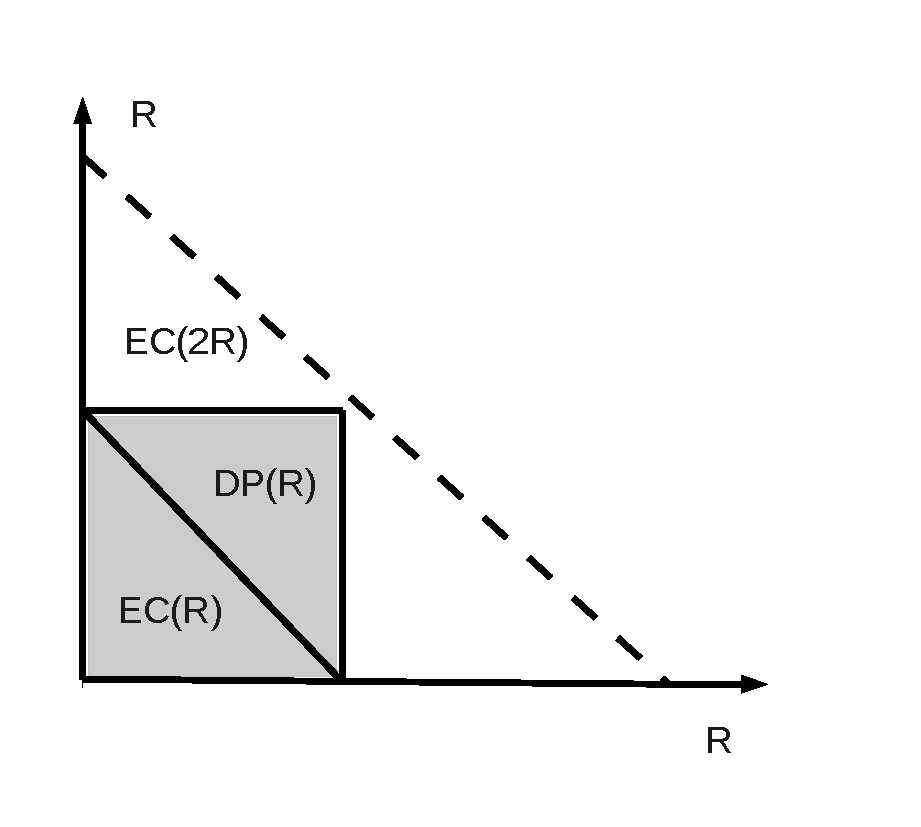
\includegraphics[scale=0.4]{../Plots/EffInt1.pdf}
\caption{Illustration of the different spaces that are involved in forming the effective interaction. The standard approach generates the interaction elements in an energy cut model space $\mathbb{EC}(R)$, corresponding to a cut in the global shell number $R$ (and energy). The SRG method uses a direct product space $\mathbb{DP}(R)$, where the single-particle shell number $R$ (and energy) is limited to a maximum. For an \textit{effective interaction without energy cut}, we use a larger energy cut model space, $\mathbb{EC}(2R)$. The term ''without energy cut'' arose because the whole direct product space $\mathbb{DP}(R)$ is included in $\mathbb{EC}(2R)$, such that there is no cut in $\mathbb{DP}(R)$.}
\label{fig:EffInt}
\end{center}
\end{figure}

In order to obtain a well-defined interaction, the effective interaction must be generated in an energy cut model space $\mathbb{EC}(R)$, see figure \ref{fig:EffInt}. In contrast to the direct product space $\mathbb{DP}(R)$, that one does not cut the single-particle shell numbers $R$ (or energy), but the global shell number.
This space $\mathbb{EC}(R)$ contains all the symmetries of the interaction and a generation in $\mathbb{DP}(R)$ would break essential symmetries like conservation of center-of-mass momentum \cite{Lohne}. Although $\mathbb{EC}(R)$ yields exact results for two particles, it has shown to have convergence problems \cite{Lohne}. Therefore the common practice arose \cite{Marte,Christoffer,Lohne,Frank} to use a basis that is twice as big, namely $\mathbb{EC}(2R)$. We will refer to the interaction in this basis as  \textit{effective interaction without energy cut}.  
Since the SRG method works in $\mathbb{DP}(R)$, we simply restrict ourselves to the interaction elements  in $\mathbb{DP}(R)$ when using an effective interaction without energy cut, which has elements generated in $\mathbb{EC}(2R)$. In the case of a large basis, the error is assumed to be fairly small, but in many cases convergence is considerably improved.


\begin{table}
\begin{center}
$N = 2$ \\
\vspace{3pt}
\begin{tabular}{c|cccc}
\hline\hline
 & &Standard  &\multicolumn{2}{c}{Effective}\\
$\omega$ &$R$ & & E-cut& No E-cut \\
\hline
 \hline   
   0.1    & 2 &  0.5125198414    &  0.440791888  & 0.4716227724  \\
          & 3 &  0.4421887603    & 0.440791888 & 0.4408841339    \\
          & 4 & 0.4418679942     & 0.440791888   &  0.4408938347   \\
          & 5 & 0.4416137068     & 0.440791888  &  0.4408701421     \\
 \hline      
   0.28   & 2 &  1.127251038    & 1.021644014  &  1.06693768    \\
          & 3 & 1.032681412     & 1.021644014   &  1.023735246  \\
          & 4 & 1.028803672     & 1.021644014  &  1.022974149          \\
          & 5 & 1.026588059     & 1.021644014    &  1.022380493       \\ 
 \hline  
   0.5   & 2 & 1.78691353      & 1.65977215&  1.71357741  \\
          & 3 & 1.681631996    & 1.65977215  &  1.664345671   \\
          & 4 & 1.673872389    & 1.65977215  &  1.662657612     \\
          & 5 & 1.669498218    & 1.65977215   & 1.661389243      \\
 \hline   
   1.0    & 2 & 3.152328007    & 3.000000000  &  3.063440415   \\
          & 3 &  3.038604576 & 3.000000000&  3.008602484   \\
          & 4 &  3.025230582   &  3.000000000  & 3.005518845      \\
          & 5 &  3.01760623    &  3.000000000   & 3.00319931    \\ 
 \hline \hline
\end{tabular}
\end{center}
\caption{Comparison of the ground state energy $E_0$ with standard and effective interaction for $N=2$ particles. The runs with effective interaction have been performed with and without energy cut, see text for further explanation. The energy is given in $[E_H]$.
  All runs have been performed with generator $\hat{\eta}_1 = \left[ \hat{T}_{\text{rel}}, \hat{V}\right]$.}
\label{tab:EffInt}
\end{table}


\begin{table}
\begin{center}
$N = 6$ \\
\vspace{3pt}
\begin{tabular}{c|c|cccc}
\hline\hline
 & &Standard  &\multicolumn{2}{c}{Effective}\\
$\omega$ &$R$ & & E-cut& No E-cut \\
 \hline
   0.1    & 3 & 4.149558313  &nc   & nc \\
          & 4 & 3.797435926  &  nc & nc  \\ 
 \hline      
   0.28   & 3 &   nc   & nc &   8.086703549 \\
          & 4 &  7.851831187  &nc  & nc   \\
 \hline  
   0.5   & 3 &   12.89722859  & nc & 12.37361922       \\
         & 4 &  12.03694209  & nc &  11.86576513   \\
 \hline   
   1.0    & 3 & 21.42058830   &nc & 20.86307299      \\  
          & 4 & 20.41582765   & nc  &  20.21066463   \\
\hline\hline
\end{tabular}
\end{center}
\caption{Comparison of the ground state energy $E_0$ (in $\left[ E_H\right]$) as in table \ref{tab:EffInt}, this time for $N=6$ particles. The label ''nc'' denotes non-converging runs.}
\label{tab:EffInt2}
\end{table}

Tables \ref{tab:EffInt} and \ref{tab:EffInt2} compare the results of a standard interaction with the ones obtained using an effective interaction. As before, all the converging runs yield precisely the same result as the exact diagonalization of the Hamiltonian does. We therefore omitted the comparison with exact diagonalization in the tables and rather focus on the relation between standard and effective interaction.\\
As stated above, the effective interaction applied to $N=2$ particles should give the same result as a standard interaction in an infinite space. Exactly as expected, we therefore observe that the result for $N=2$ particles with energy cut does not change as the number of shells $R$ is increased. Moreover, we reproduce $E_0 = 3$ (in $\left[ E_H \right]$) for $N=2$ electrons and $\omega = 1.0$, which is the exact result that has been analytically derived \cite{PhysRevA.48.3561}. \\
Although the effective interaction without energy cut is less exact, table \ref{tab:EffInt} shows that it is numerically much more stable.  With energy cut, the convergence behaviour turned out to be worth
than with standard interaction, therefore we will use the effective interaction only without energy cut from now on. This decision has also be made by previous and fellow master students studying quantum dots with Full Configuration Interaction \cite{Frank} and Coupled Cluster \cite{Christoffer} and will therefore enable us to directly compare results in section \ref{sec:IMSRGres}.

Table \ref{tab:EffInt} and figure \ref{fig:stdeff} illustrate that the effective interaction gives a better convergence for the ground state energy as function of shell numbers $R$. However, it does not seem to lead to a considerable improvement of integrator's numerical stability. The convergence is getting worse as the oscillator frequency $\omega$ is decreasing as the number of particles $N$ is getting larger, which indicates that a higher correlation between the electrons is responsible for the numerical instability.

\begin{figure}
\begin{center}
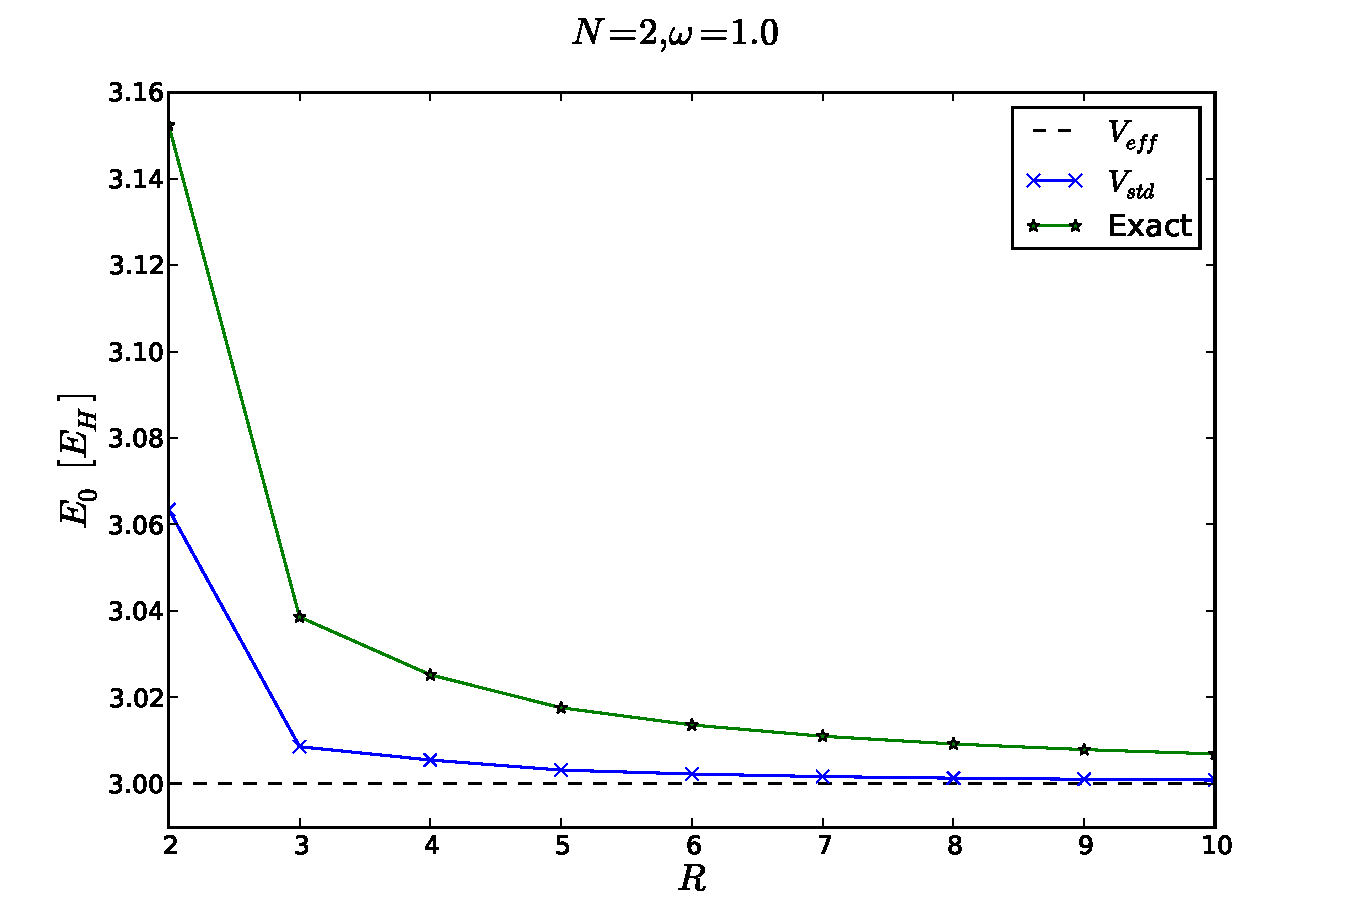
\includegraphics[scale=0.4]{../Plots/stdeff.pdf}
\end{center}
\caption{Comparison between standard and effective interaction (without energy cut) for $N=2$ particles. With increasing number of shells $R$, the ground state energy $E_0$ converges towards the analytically exact result. The convergence with effective interaction is faster and the result for a given $R$ a better approximation for $E_0$ than with standard interaction.}
\label{fig:stdeff}
\end{figure}

\subsubsection{Hartree-Fock basis}
Since changing the interaction has not resulted in an improved numerical stability, we hope to solve this problem by replacing the harmonic oscillator by a Hartree-Fock basis. After the Hartree-Fock calculation, the one-particle-one-hole excitations will be zeroed out. Since those ones are assumed to have greatest impact on the electron interaction, we hope to have fewer problems due to high correlations.

A first important result is that runs with a Hartree-Fock basis give the same result as runs with a harmonic oscillator basis. This is demonstrated in table \ref{tab:HFtest} , where we performed tests with $N=2$ particles and different values of $R$ and $\omega$.\\
Since a basis transformation should preserve physical observables like energy, this confirms our expectations and implies that the Hartree-Fock method is correctly implemented. Additionally, we have shown that the SRG method is also stable with a Hartree-Fock basis and converges to the correct results.

\begin{table}
{\small
\begin{center}
$N=2,\,\omega = 1.0$
\vspace{11pt}
\begin{tabular}{|c||c|c|c||c|c|c|}
\hline
  & \multicolumn{3}{|c||}{Standard} & \multicolumn{3}{|c|}{Effective}\\
$R$ & 2& 5& 10& 2 & 5 & 10  \\
\hline
HO basis &3.152328007 &3.01760623 & 3.006937178 & 3.063440415 &3.00319931 & 3.000894294\\
\hline
HF basis & 3.152328007 &3.01760623 &3.006937178 &3.063440415 &3.00319931 & 3.000894294\\
\hline
\end{tabular}

$N=2,\,\omega = 0.1$
\vspace*{5pt}
{\tabcolsep=0.12cm
\begin{tabular}{|c||c|c|c||c|c|c|}
\hline
  & \multicolumn{3}{|c||}{Standard} & \multicolumn{3}{|c|}{Effective}\\

$R$ & 2& 5& 10& 2 & 5 & 10  \\
\hline 
HO basis &  0.5125198414&0.4416137068 &0.441135127  &0.4716227724  & 0.4408701421&  0.4408186851\\
\hline
HF basis & 0.5125198414 & 0.4416137068 &0.441135127 & 0.4716227724& 0.4408701421 &  0.4408186851 \\
\hline
\end{tabular}
}
\end{center}
}
\caption{Comparison of the ground state energy $E_0$ (in $\left[ E_H \right]$) obtained with a harmonic oscillator (HO) and a Hartree-Fock (HF) basis. The large number of  specified decimals shall demonstrate that a Hartree-Fock basis reproduces exactly the same results.}
\label{tab:HFtest}
\end{table}

\begin{figure}
\begin{center}
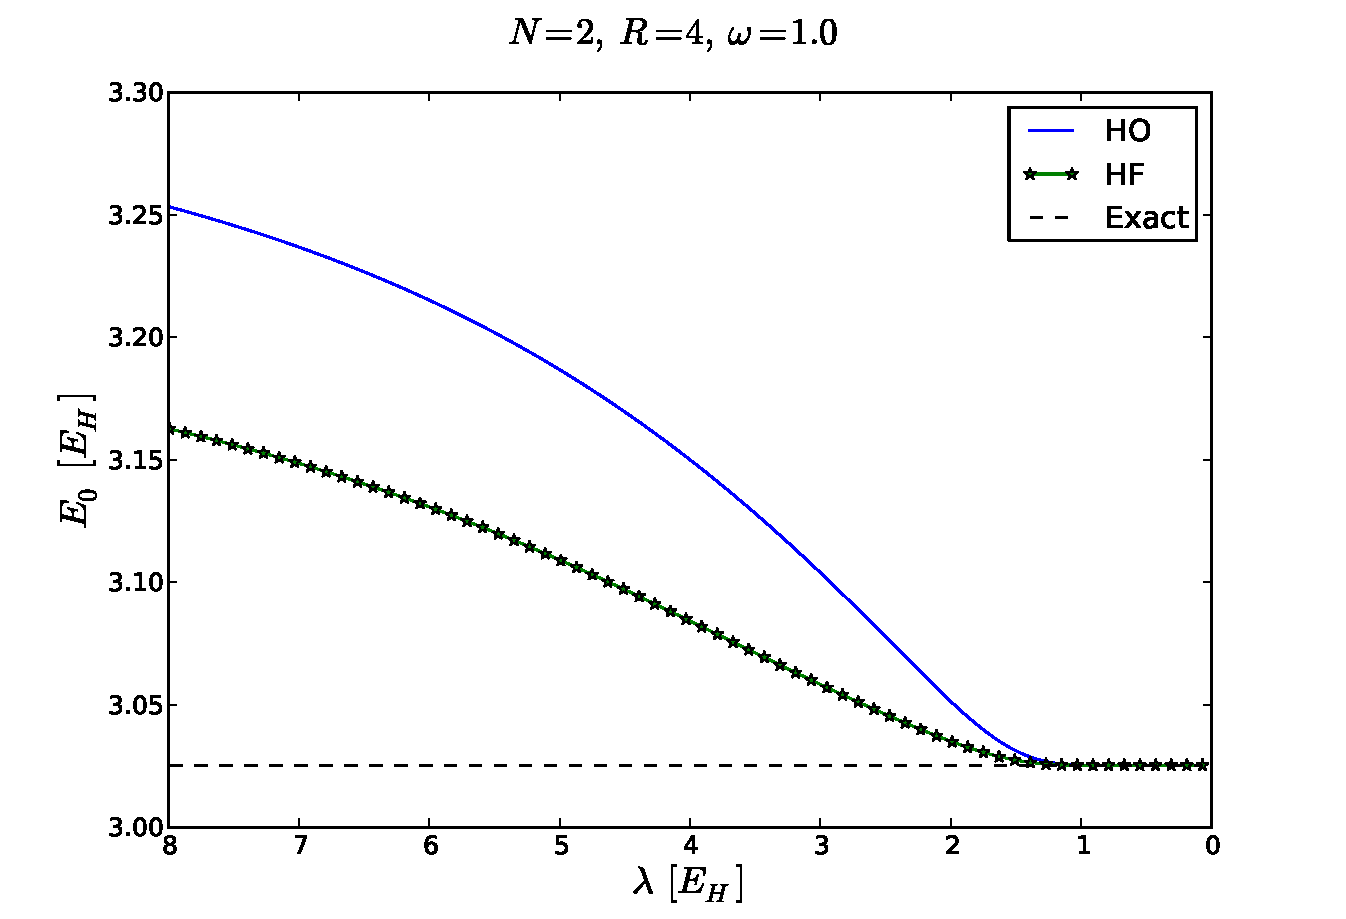
\includegraphics[scale=0.4]{../Plots/HOHF.pdf}
\end{center}
\caption{Comparison of the convergence behaviour for a harmonic oscillator (HO) and a Hartree-Fock (HF) basis. With a HF basis, the one-particle-one-hole excitations are already zeroed out from the beginning, such that the ground state energy $E_0$ starts with a lower value. The plot shows a system with standard interaction and $\hat{\eta}_1 = \left[ \hat{T}_{\text{rel}}, \hat{V}\right]$. }
\label{fig:HOHF}
\end{figure}


Having verified that, in the case of convergence, the basis transformation reproduces the earlier obtained results, we focus on the so far non-converging results and analyse whether convergence is improved with a Hartree-Fock basis. Since generator $\hat{\eta}_1 = \left[ T_{\text{rel}}, \hat{V}\right]$ yielded better numerics, we will limit ourselves to this generator.



\begin{table}
\begin{center}
\subtable[Standard Interaction, $N=6$]{
\begin{tabular}{|c|c|cc|}
\hline\hline
 $\omega$ & $R$ & HO basis & HF basis \\
\hline
 0.1 & 3 & nc & nc \\
 &  4 & nc & nc \\ 
      \cline{1-4}
  0.15 & 3 & nc & nc \\
  0.2 & 3 & nc & nc \\
  0.28 & 3 & nc & nc \\ 
\hline\hline
\end{tabular}
\vspace{11pt}
}
\subtable[Effective Interaction, $N=6$ ]{
\begin{tabular}{|c|c|cc|}
\hline\hline
 $\omega$ & $R$ & HO basis & HF basis \\
\hline
 0.1 &  3 & nc & nc \\
      &  4 & nc & nc \\ 
      \cline{1-4}
  0.15 & 3 & nc & nc\\
  0.2 & 3 & nc & nc\\
  0.28 & 4 & nc & 7.703042 \\ 
\hline\hline
\end{tabular}
}

\end{center}
\caption{Runs not converging with a harmonic oscillator (HO) basis are repeated with a Hartree-Fock (HF) basis. For the converging cases, the ground state energy $E_0$ is given in $\left[E_H\right]$.}
\label{tab:HOvsHF}
\end{table}

Table \ref{tab:HOvsHF} summarizes the results: With a standard interaction, we have not gotten any improvement. For low oscillator frequencies $\omega$, the numerical integration is still unstable, resulting in a non-converging ground state energy. With an effective interaction, the stability has not considerably improved, either. Just in one case, the basis transformation could resolve the numerical problem.

From studies of two-dimensional quantum dots with the Coupled Cluster method \cite{Marte,Christoffer,Lohne}, we know that convergence sometimes gets better as the number of shells $R$ is increased. Since an increase of $R$ also corresponds to a better result since higher correlations are included, these cases are of higher interest, anyway. We therefore hope to obtain a better convergence pattern by including more basis states. However, due to its high demands on CPU time and memory, the free-space SRG method is not the method of choice in these cases. We will rather take benefit of the advantages of in-medium SRG and use this method study systems with a larger number basis states.


\subsection{Time analysis}

The advantage of the SRG method in free space is that no truncation is made and, apart from non-converging cases, the same result is obtained as for exact diagonalization. However, this requires to set up the full Hamiltonian matrix, which with increasing number of basis states gets exceedingly large.

\begin{table}
\begin{center}
\begin{tabular}{c| c c c}
\hline
 $N$ & $R=3$ & $R = 5$ & $R = 7$ \\
 \hline
  2  & 8 & 29 & 72\\
  6  & 64 & 16451 & 594118\\
 12  & - & 1630953& 579968 \\ 
 \hline
\end{tabular}
\end{center}
\caption{Number $n$ of relevant basis states in M-scheme with constraint $M = M_s = 0$.}
\label{tab:numBasis}
\end{table}

Table \ref{tab:numBasis} illustrates how the number of Slater determinants with the constraint $M = M_s = 0$ is rapidly increasing with the number of particles $N$ and shells $R$. One the one hand, this might quickly exceed the available memory to store the full $n\times n$ Hamiltonian matrix. On the other hand, the computational cost gets unacceptably high since each call of the derivative function (\ref{eq:flow}) is of order $\mathcal{O}(n^3/2)$. The latter reason made us limit to rather small systems in table \ref{tab:free2}. To get an impression of the required CPU time of such a run, table \ref{tab:timeAnalysis} lists how much time is needed for a system with $N=6$ particles on $R=4$ shells in order to obtain the ground state energy $E_0$ up to a certain accuracy. Together with figure \ref{fig:time1}, it gets obvious that especially the last part of the flow, i.e. the last correct digits, are very CPU demanding. \\


\begin{table}
\begin{center}
\begin{tabular}{c c c}
\hline\hline
 $\lambda$ & $E_0$ & CPU time in $s$ \\
 \hline
 20.0 & \textbf{2}2.20366072 & 660 \\
% 17.0 & 22.18361918 & 1320 \\
 10.0 & \textbf{2}2.05448854 & 1756 \\
% 5.0 & \textbf{2}1.59433320 & 2387  \\
 3.0  & \textbf{2}0.99839817 & 2908  \\
 2.0  & \textbf{20}.57836962 & 3363 \\
 1.4  & \textbf{20.4}3153289 & 4608 \\
 1.0 & \textbf{20.416}04434 & 6813 \\
 0.8 & \textbf{20.41582}988 & 9126 \\
 0.6 & \textbf{20.41582765} & 14039 \\
\hline\hline
\end{tabular}
\end{center}
\caption{The table lists the required CPU time for different values of the flow evolution parameter $\lambda$. The corresponding ground state energy $E_0$  is given in units of $\left[E_H\right]$, from $\lambda = s^{-1/2}$ follows that $\left[\lambda\right] = \left[ E \right]$. The studied system consists of $N=6$ particles on $R=4$ shells with $\omega=1.0$ and $\hat{\eta}_1 = \left[ \hat{T}_{\text{rel}}, \hat{V}\right]$. The interaction is a standard Coulomb one, and the basis is modelled by a harmonic oscillator basis. The bold letters indicate correct digits with respect to exact diagonalization. }
\label{tab:timeAnalysis}
\end{table}

\begin{figure}
\begin{center}
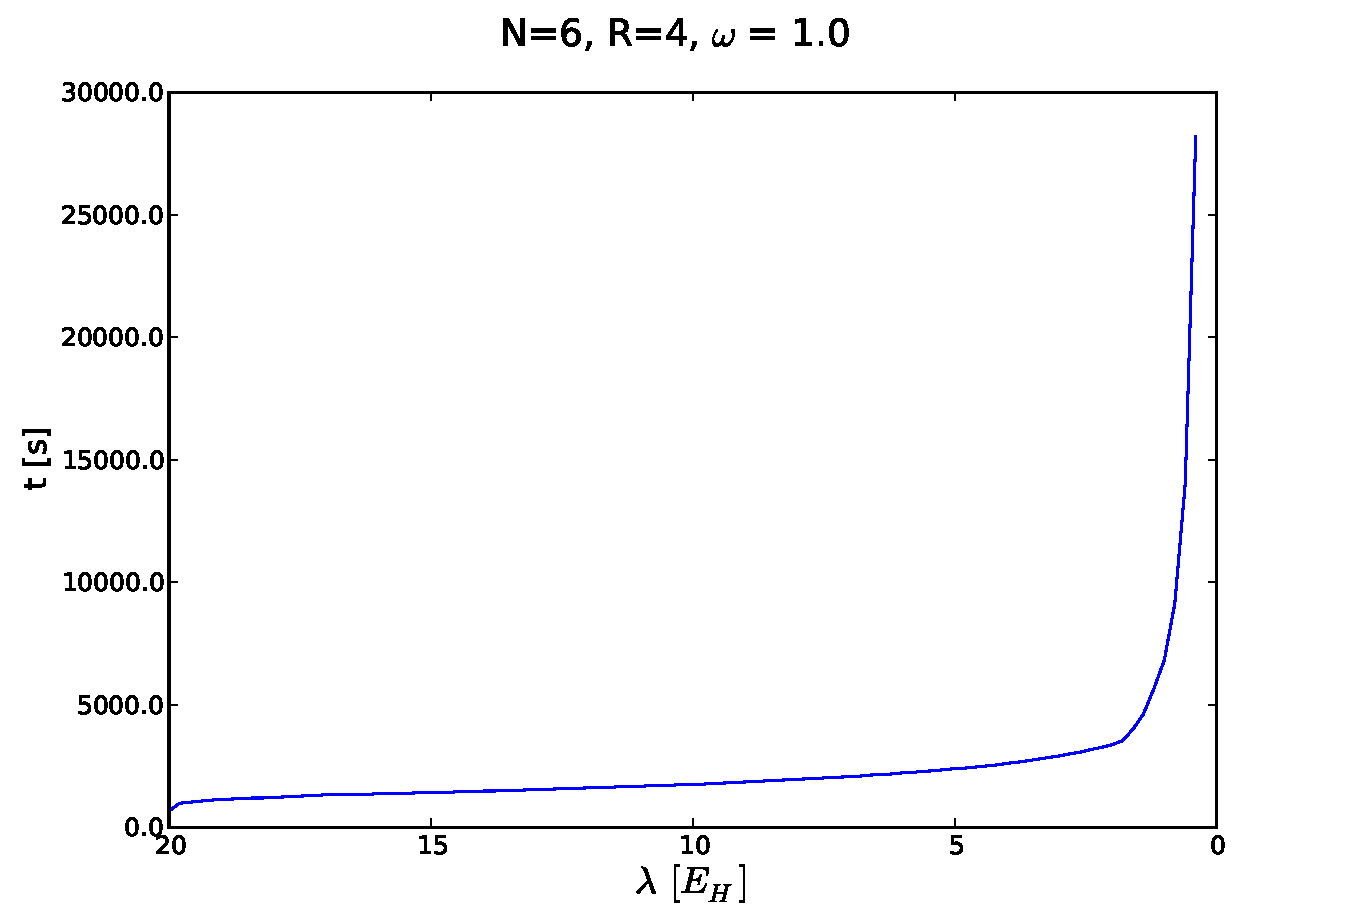
\includegraphics[scale=0.35]{../Plots/time1.pdf}
\caption{Required CPU time as function of the flow parameter $\lambda$. The example is for $N=6$ particles on $R=4$ shells and $\hat{\eta}_1 = \left[ \hat{T}_{\text{rel}}, \hat{V}\right]$.}
\label{fig:time1}
\end{center}
\end{figure}

Analysing the program explicitly, we have found out that for larger systems more than $90$\% of the CPU time is spent computing the derivatives. This percentage is even increasing as the dimension $n$ of the Hamiltonian gets larger.\\
The problem with the free-space approach up to this point is that, we in fact do diagonalize the full Hamiltonian matrix, but with a method that demands much more floating point operations than advanced iterative diagonalization methods like the Lanczos algorithm do. We remind that each computation of the flow derivatives (\ref{eq:flow}) is of order $\mathcal{O}(n^3/2)$.\\
If we diagonalize the example of table \ref{tab:timeAnalysis} with the standard diagonalization routine of the Armadillo library, the needed CPU time is $3$s, which is five orders of magnitude smaller than the corresponding SRG time to obtain an accuracy of ten correct digits.\\
Although the method itself gives very promising results, this time analysis emphasizes the need for another approach, the in-medium SRG method.
